\documentclass[a4paper,12pt]{report}
\usepackage[utf8]{inputenc}
\usepackage[T5]{fontenc}
\usepackage[vietnamese]{babel}
\usepackage{graphicx}
\usepackage{amsmath}
\usepackage{amssymb}
\usepackage{amsfonts}
\usepackage{hyperref}
\usepackage{geometry}
\usepackage{float}
\usepackage{caption}
\usepackage{subcaption}
\usepackage{algorithm}
\usepackage{algorithmic}
\usepackage{setspace}
\geometry{a4paper, margin=2.5cm}

\onehalfspacing

\begin{document}

\begin{titlepage}
    \centering
    \vspace*{2cm}
    \Large \textbf{TRƯỜNG ĐẠI HỌC KHOA HỌC TỰ NHIÊN}\\
    \Large \textbf{KHOA TOÁN - CƠ - TIN HỌC}\\
    \vspace{1cm}
    \LARGE \textbf{NHẬN DIỆN TỪ VỰNG NGÔN NGỮ KÝ HIỆU SỬ DỤNG MẠNG NƠ-RON ĐỒ THỊ KHÔNG GIAN - THỜI GIAN (ST-GCN)}\\
    \vspace{2cm}
    \Large \textbf{Sinh viên thực hiện:}\\
    \vspace{0.5cm}
    \textit{Đặng Xuân Minh Hiếu - 24002005}\\
    \vspace{1cm}
    \textit{Mai Hoàng Đức - 22001565}\\
    \textit{Lê Quý Công - 22001550}\\
    \vspace{1cm}
    \Large \textbf{Giảng viên hướng dẫn:}\\
    \vspace{0.5cm}
    \textit{TS. Cao Văn Chung}\\
    \vfill
    \Large \textbf{Hà Nội, Năm 2026}
\end{titlepage}

\tableofcontents
\listoffigures
\listoftables
\newpage

\chapter*{Mở đầu}
\addcontentsline{toc}{chapter}{Mở đầu}

\section*{Tính cấp thiết của Đề tài}
Sự bùng nổ của trí tuệ nhân tạo (AI) trong những thập kỷ gần đây đã mang lại vô số giải pháp công nghệ nhằm hỗ trợ đời sống con người. Các mô hình nhận dạng giọng nói (Speech Recognition) và dịch thuật tự động (Machine Translation) đã trở nên phổ biến và đạt hiệu suất vượt trội. Tuy nhiên, ngôn ngữ ký hiệu (Sign Language) vẫn còn gặp rất nhiều rào cản trong việc giao tiếp.

\section*{Các thách thức trong Bài toán WSLR}
Trong lịch sử phát triển của AI, các kỹ thuật dùng Convolutional Neural Networks (CNN) 2D hoặc 3D đã được áp dụng rộng rãi trên chuỗi hình ảnh RGB thô. Tuy nhiên, phương pháp này gặp phải các nhược điểm về độ nhiễu môi trường và chi phí tính toán khổng lồ. Báo cáo này đề xuất sử dụng MediaPipe và mạng ST-GCN để vượt qua các thách thức này.

\chapter{Tổng quan Tài liệu và Cơ sở Lý thuyết}

\section{Tổng quan Tài liệu}
Skeleton-based Action Recognition tập trung vào việc mô tả hành động thông qua quỹ đạo chuyển động của các khớp xương 3D. Yan et al. (2018) đã đề xuất mạng \textbf{ST-GCN}, biểu diễn cơ thể người như một đồ thị.

\section{Trích xuất Đặc trưng với MediaPipe Tasks API}
Thay vì sử dụng các pipeline cũ, đồ án này sử dụng \textbf{MediaPipe Tasks API} (bao gồm \texttt{pose\_landmarker} và \texttt{hand\_landmarker}) để trích xuất 75 điểm mốc (33 Pose, 21 Tay trái, 21 Tay phải) với độ chính xác cao và độ trễ thấp.

\begin{figure}[H]
    \centering
    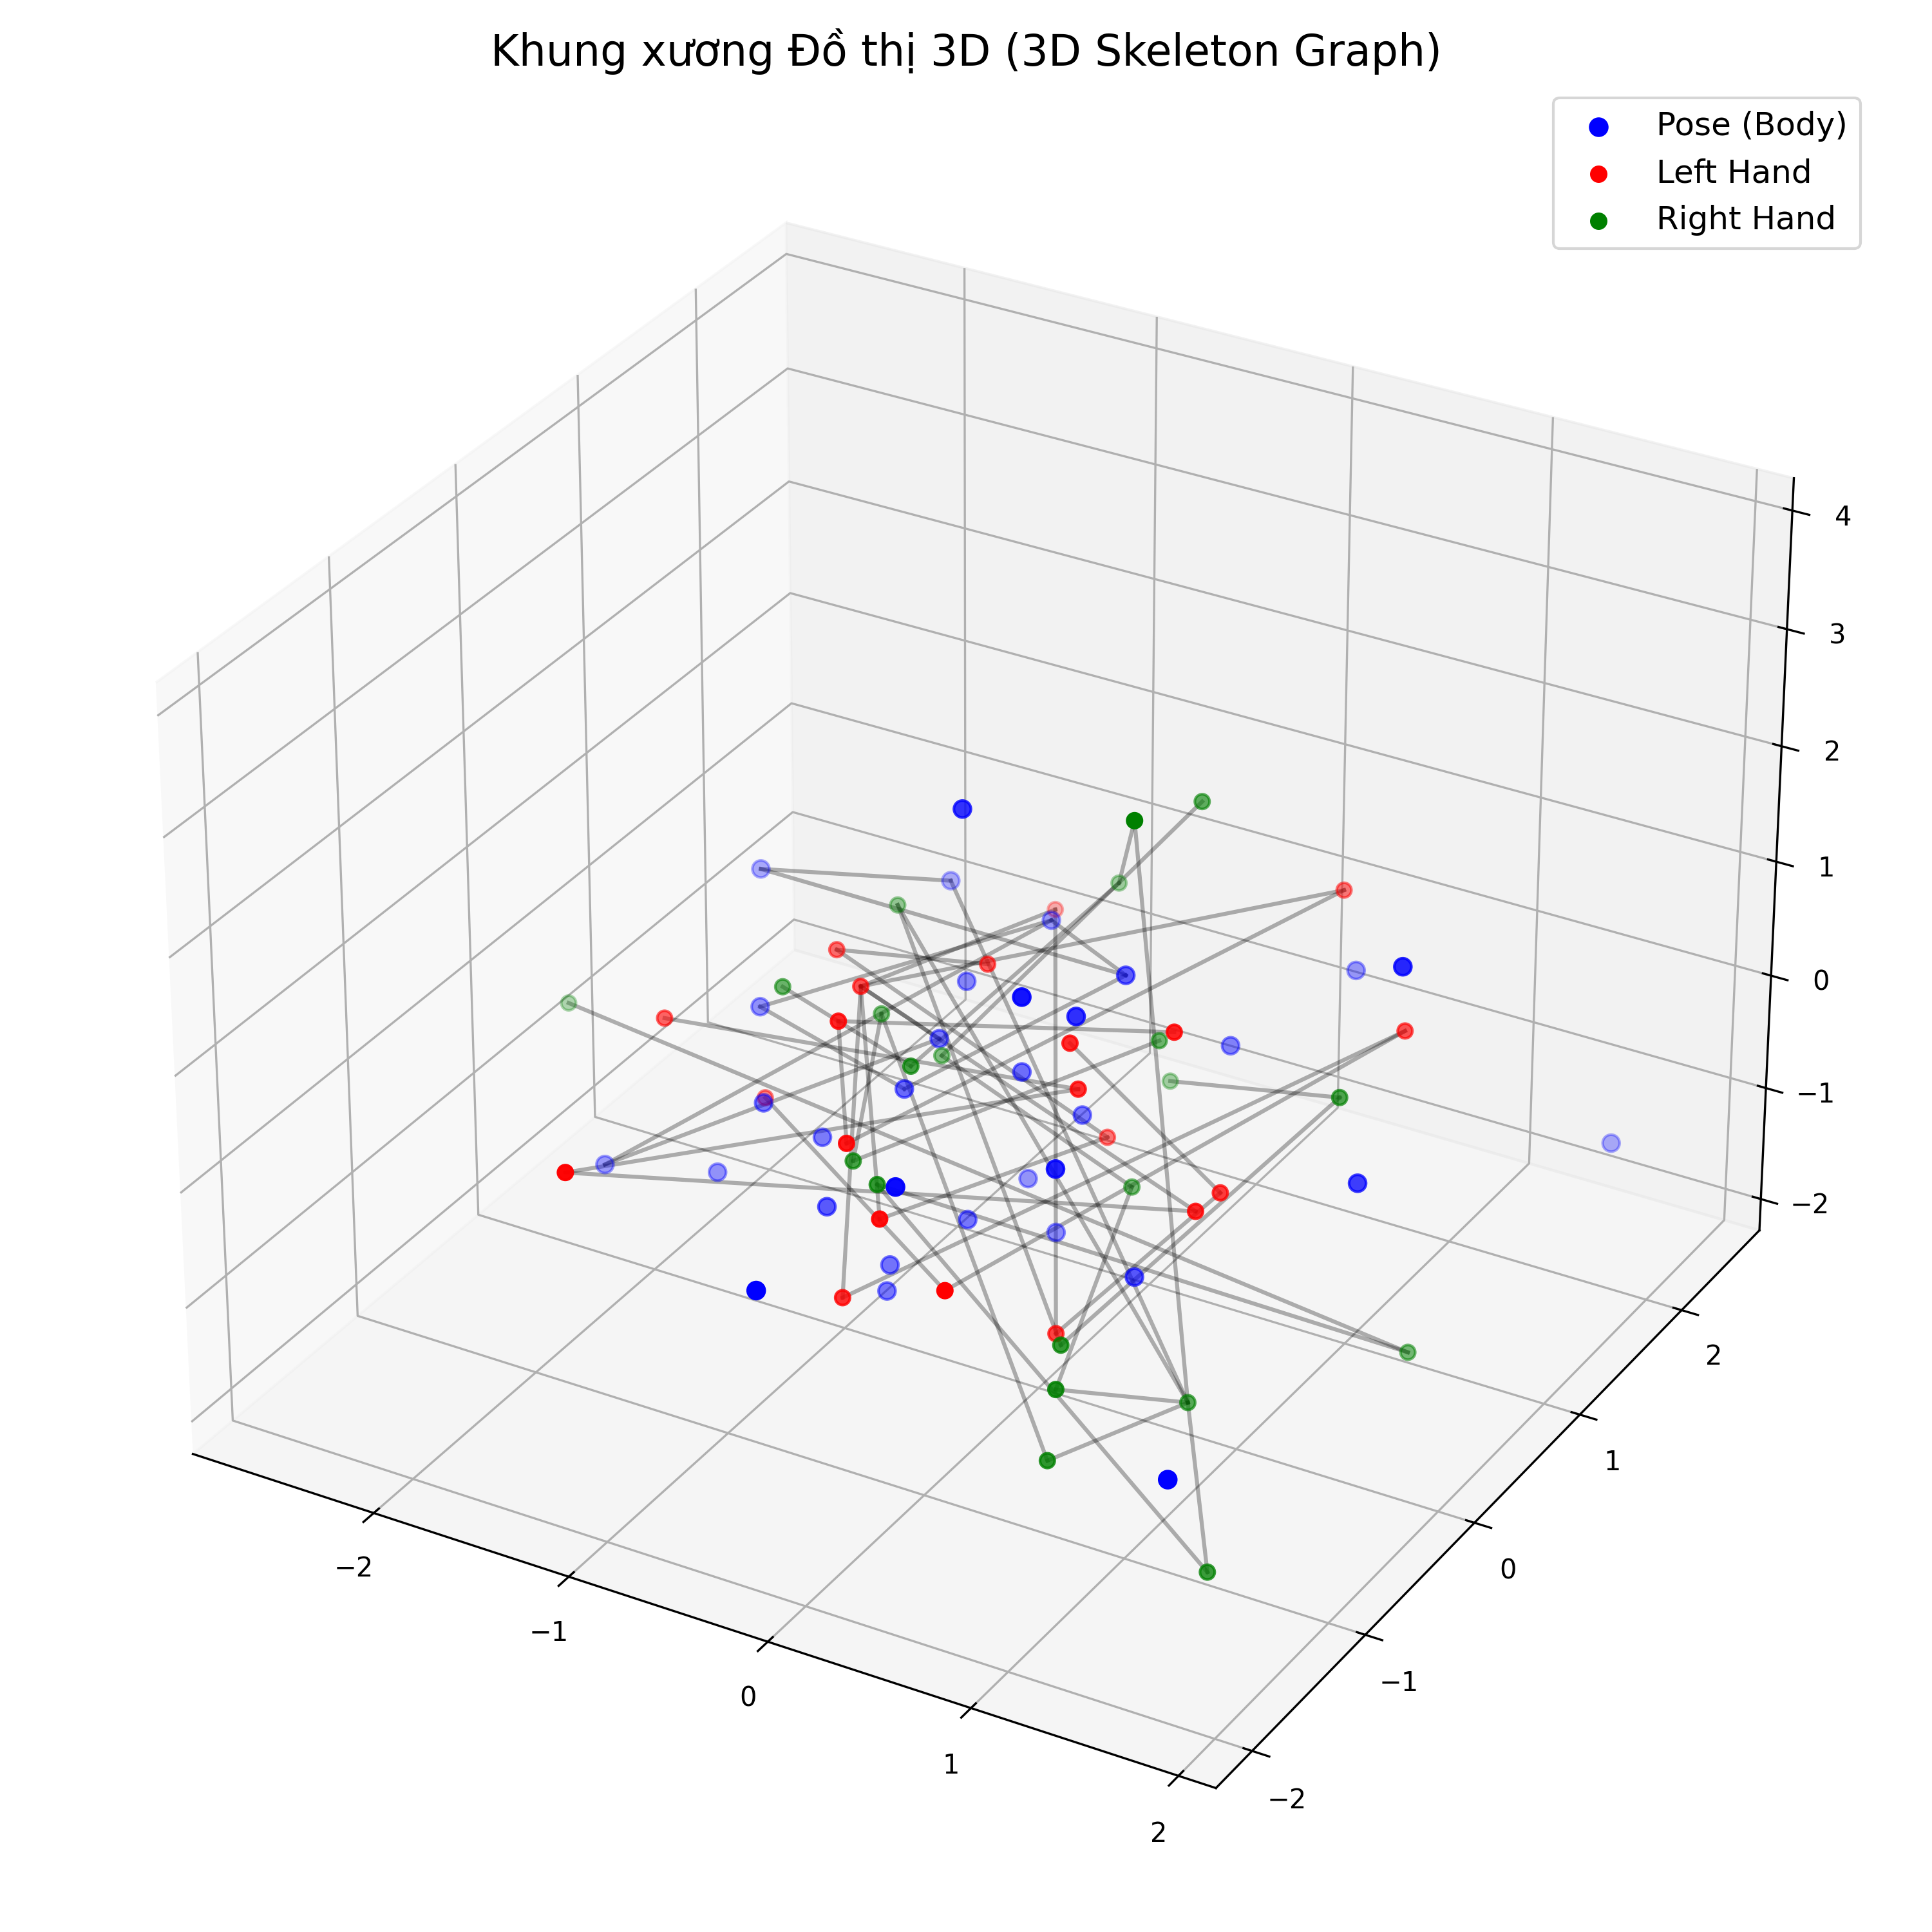
\includegraphics[width=0.7\textwidth]{report/images/skeleton_3d.png}
    \caption{Phác họa Cấu trúc liên kết của Khung xương 3D.}
    \label{fig:3d_skeleton}
\end{figure}

\section{Lý thuyết Mạng nơ-ron Đồ thị và ST-GCN}
Một đồ thị $\mathcal{G} = (V, E)$ được xác định bởi các đỉnh $V$ và cạnh $E$. Phép tích chập đồ thị sử dụng ma trận kề chuẩn hóa.

\begin{figure}[H]
    \centering
    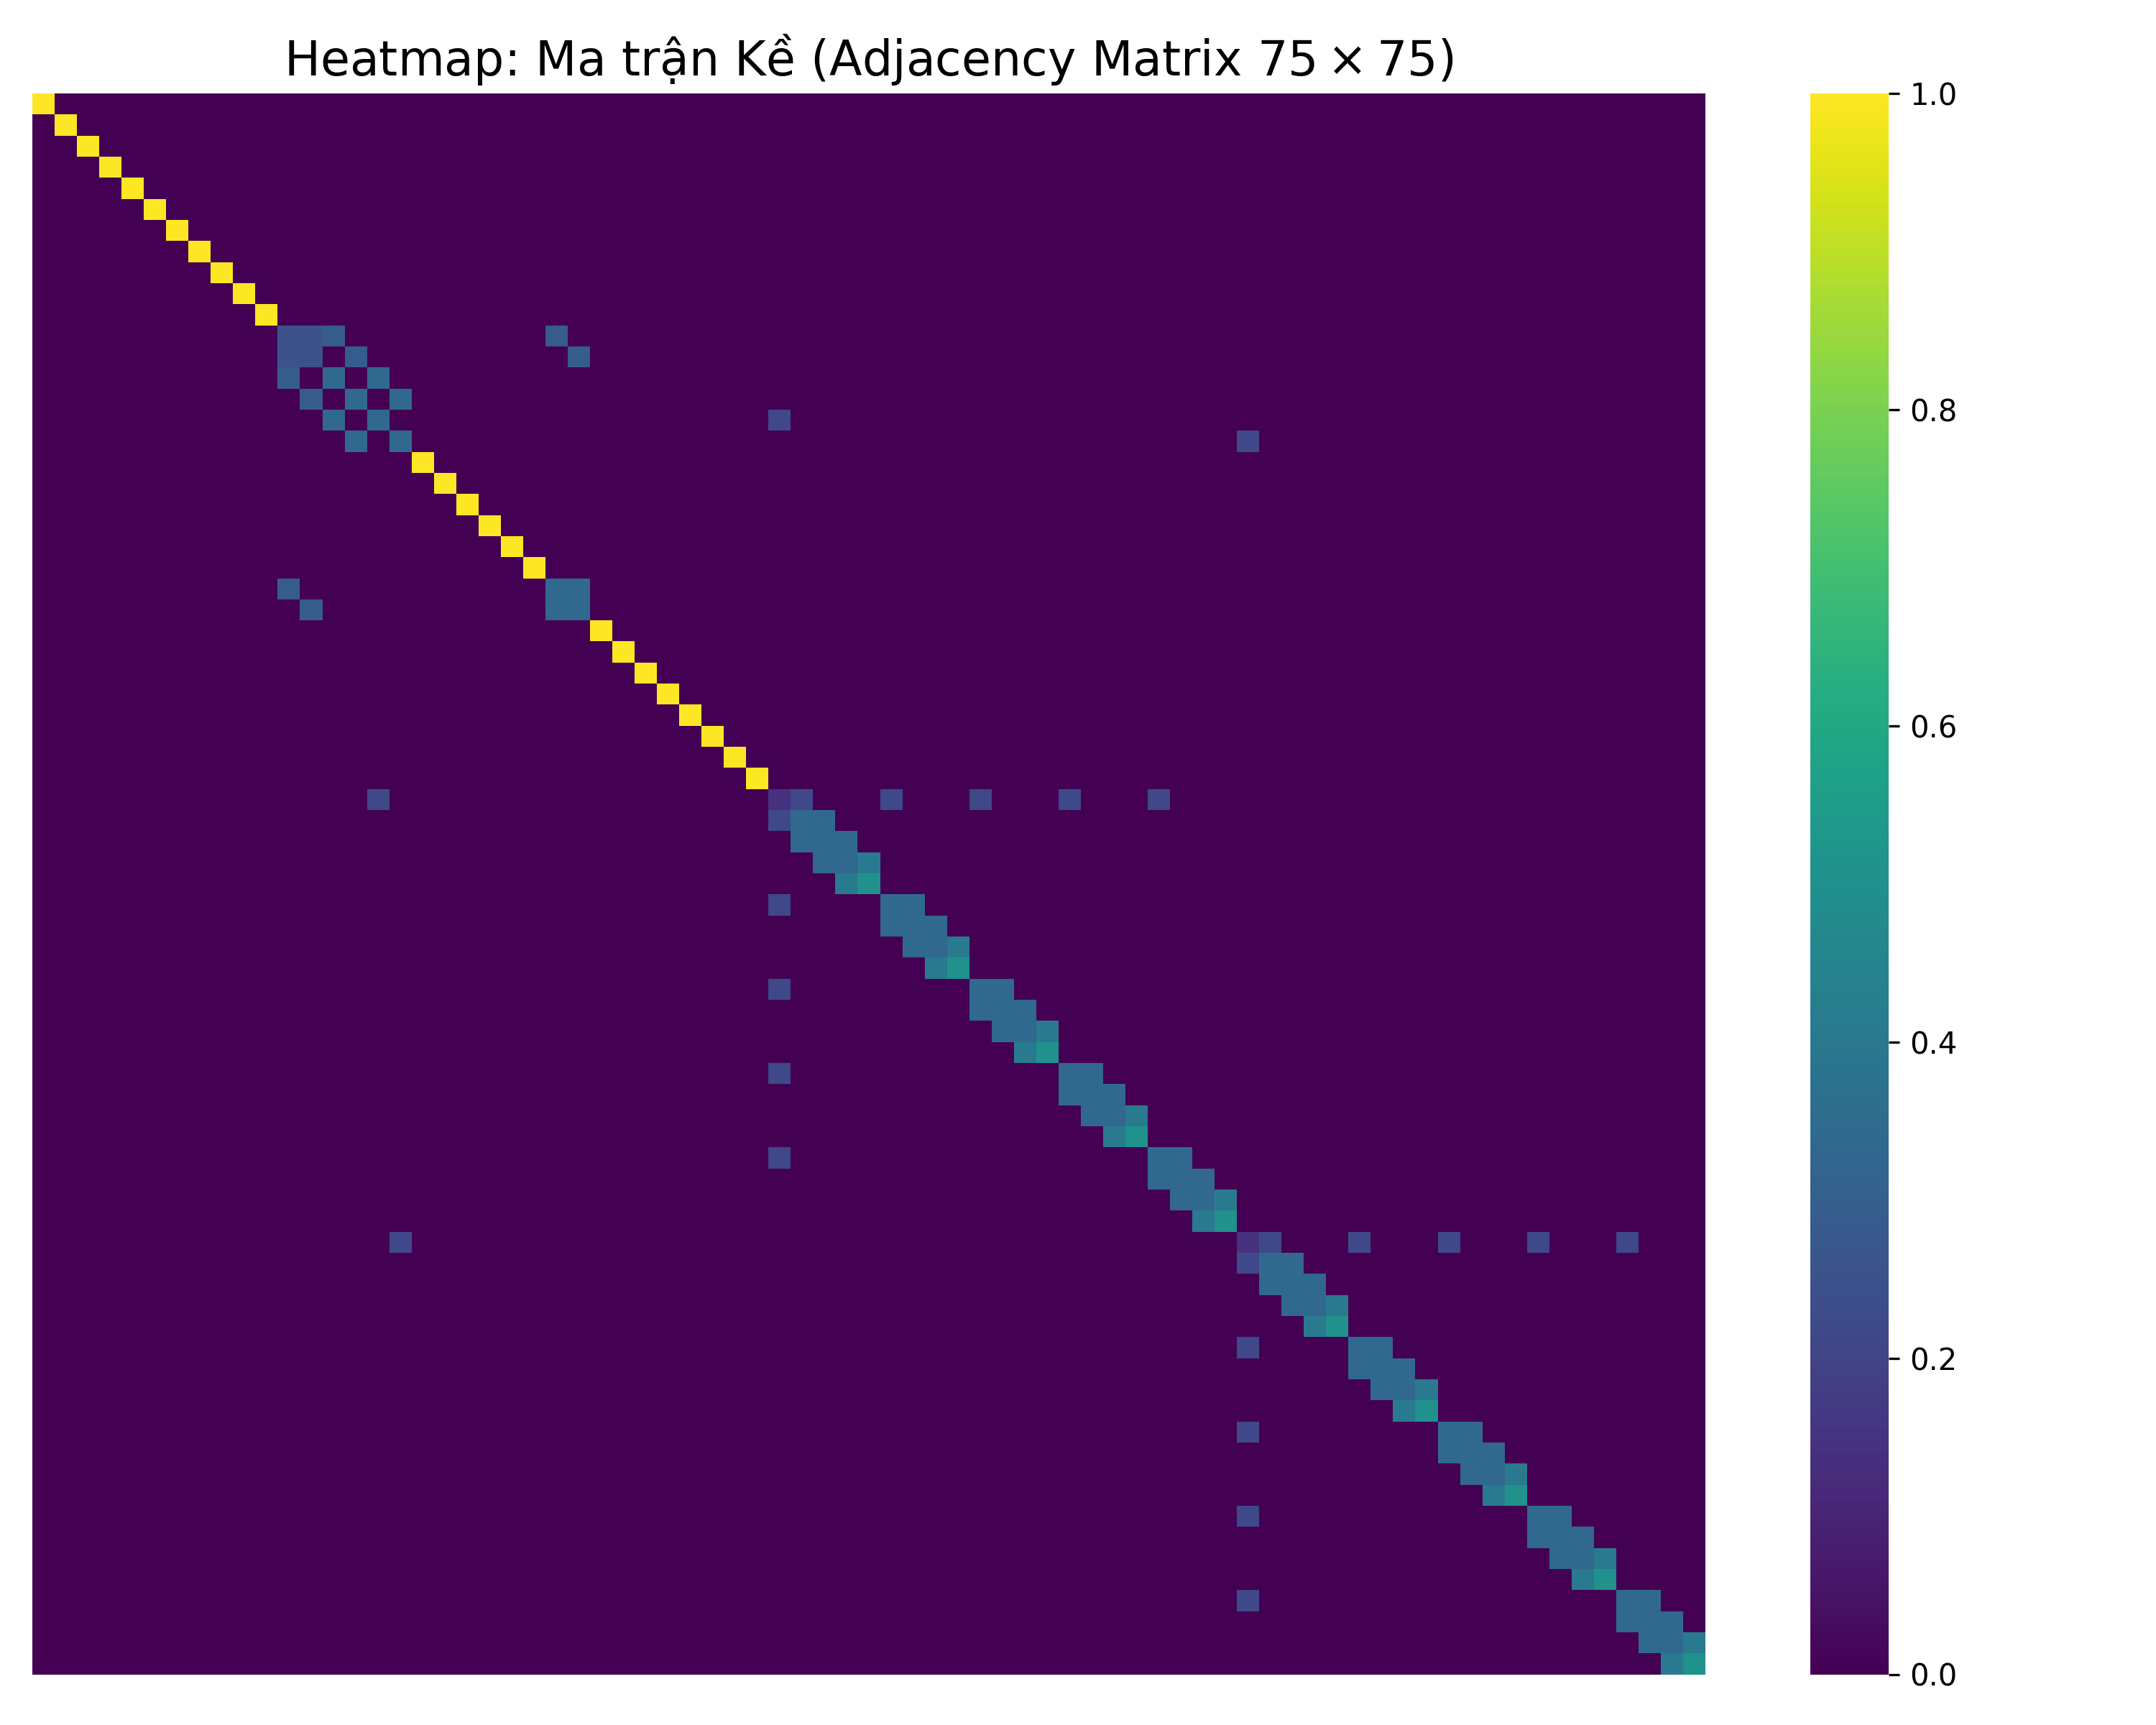
\includegraphics[width=0.7\textwidth]{report/images/adjacency_heatmap.png}
    \caption{Heatmap trực quan hóa Ma trận Kề $A$.}
    \label{fig:adjacency}
\end{figure}

\chapter{Phương pháp đề xuất và Kiến trúc hệ thống}

\section{Tiền xử lý và Phân tích Dữ liệu (EDA)}
Dữ liệu WLASL-100 được chuẩn hóa về độ dài $T=60$ frames và chuẩn hóa không gian theo vị trí Mũi và khoảng cách vai.

\begin{figure}[H]
    \centering
    \begin{subfigure}[b]{0.45\textwidth}
        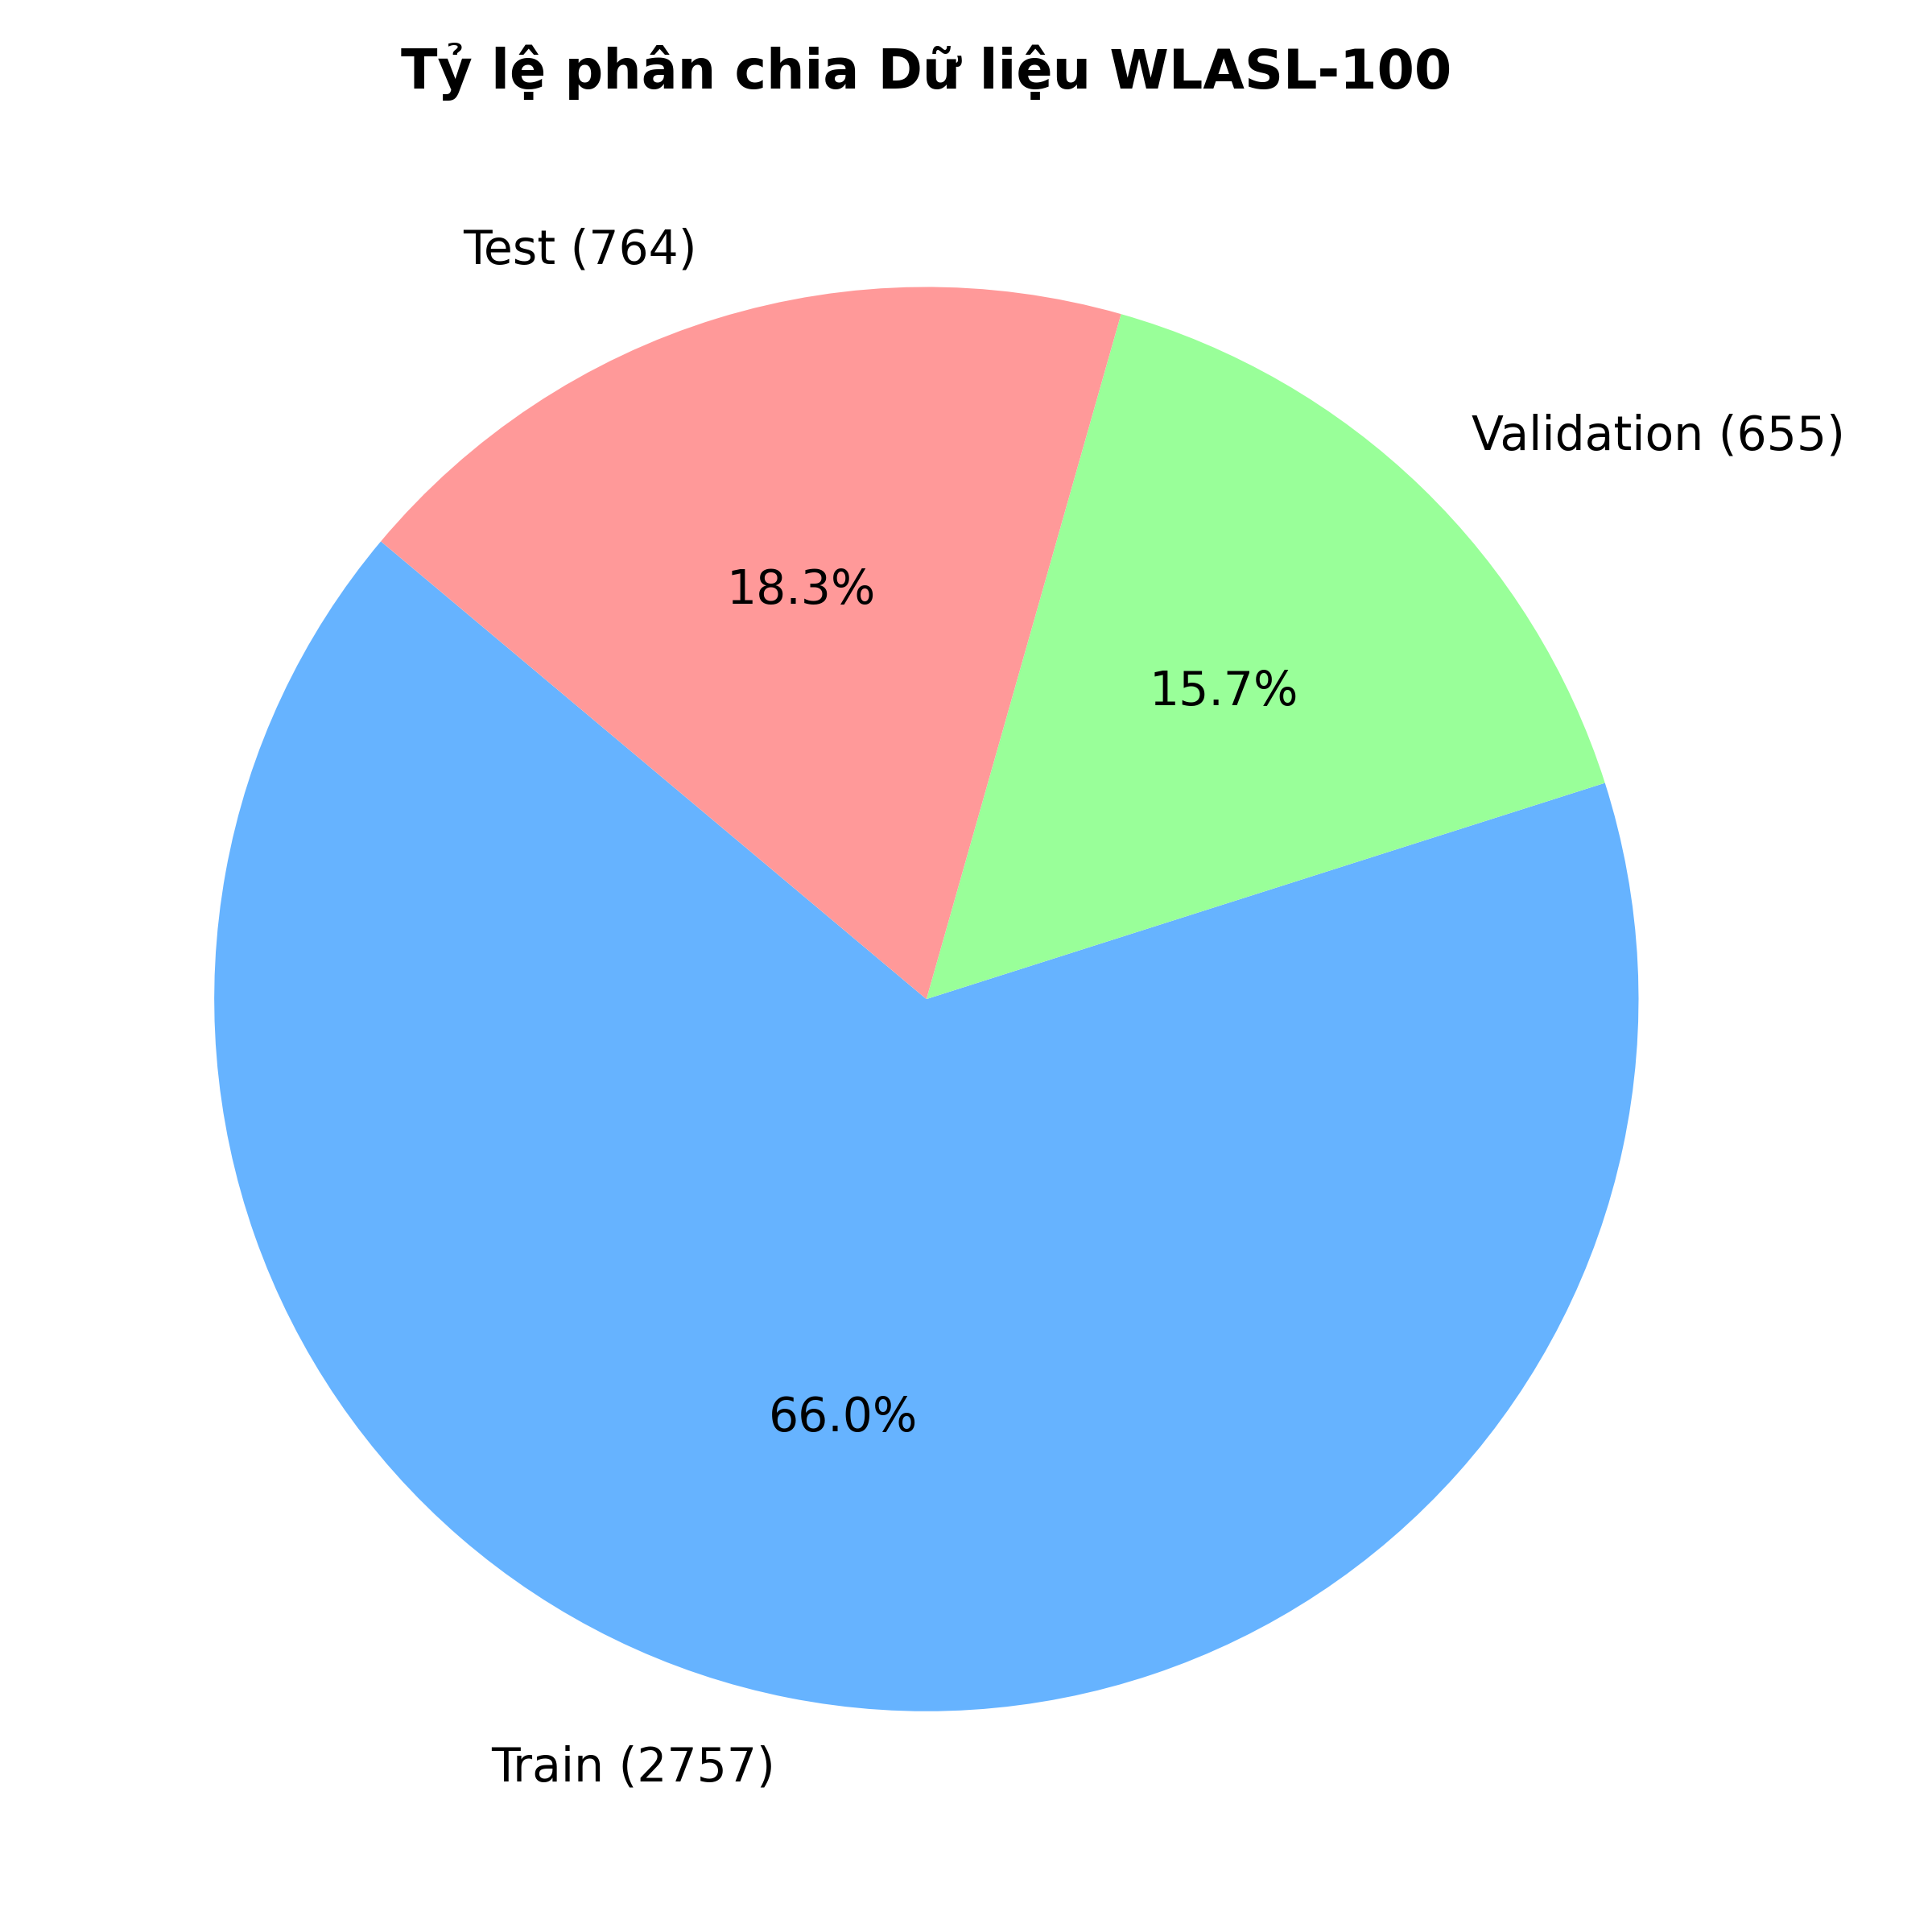
\includegraphics[width=\textwidth]{report/images/dataset_pie.png}
        \caption{Phân chia tập dữ liệu.}
    \end{subfigure}
    \hfill
    \begin{subfigure}[b]{0.45\textwidth}
        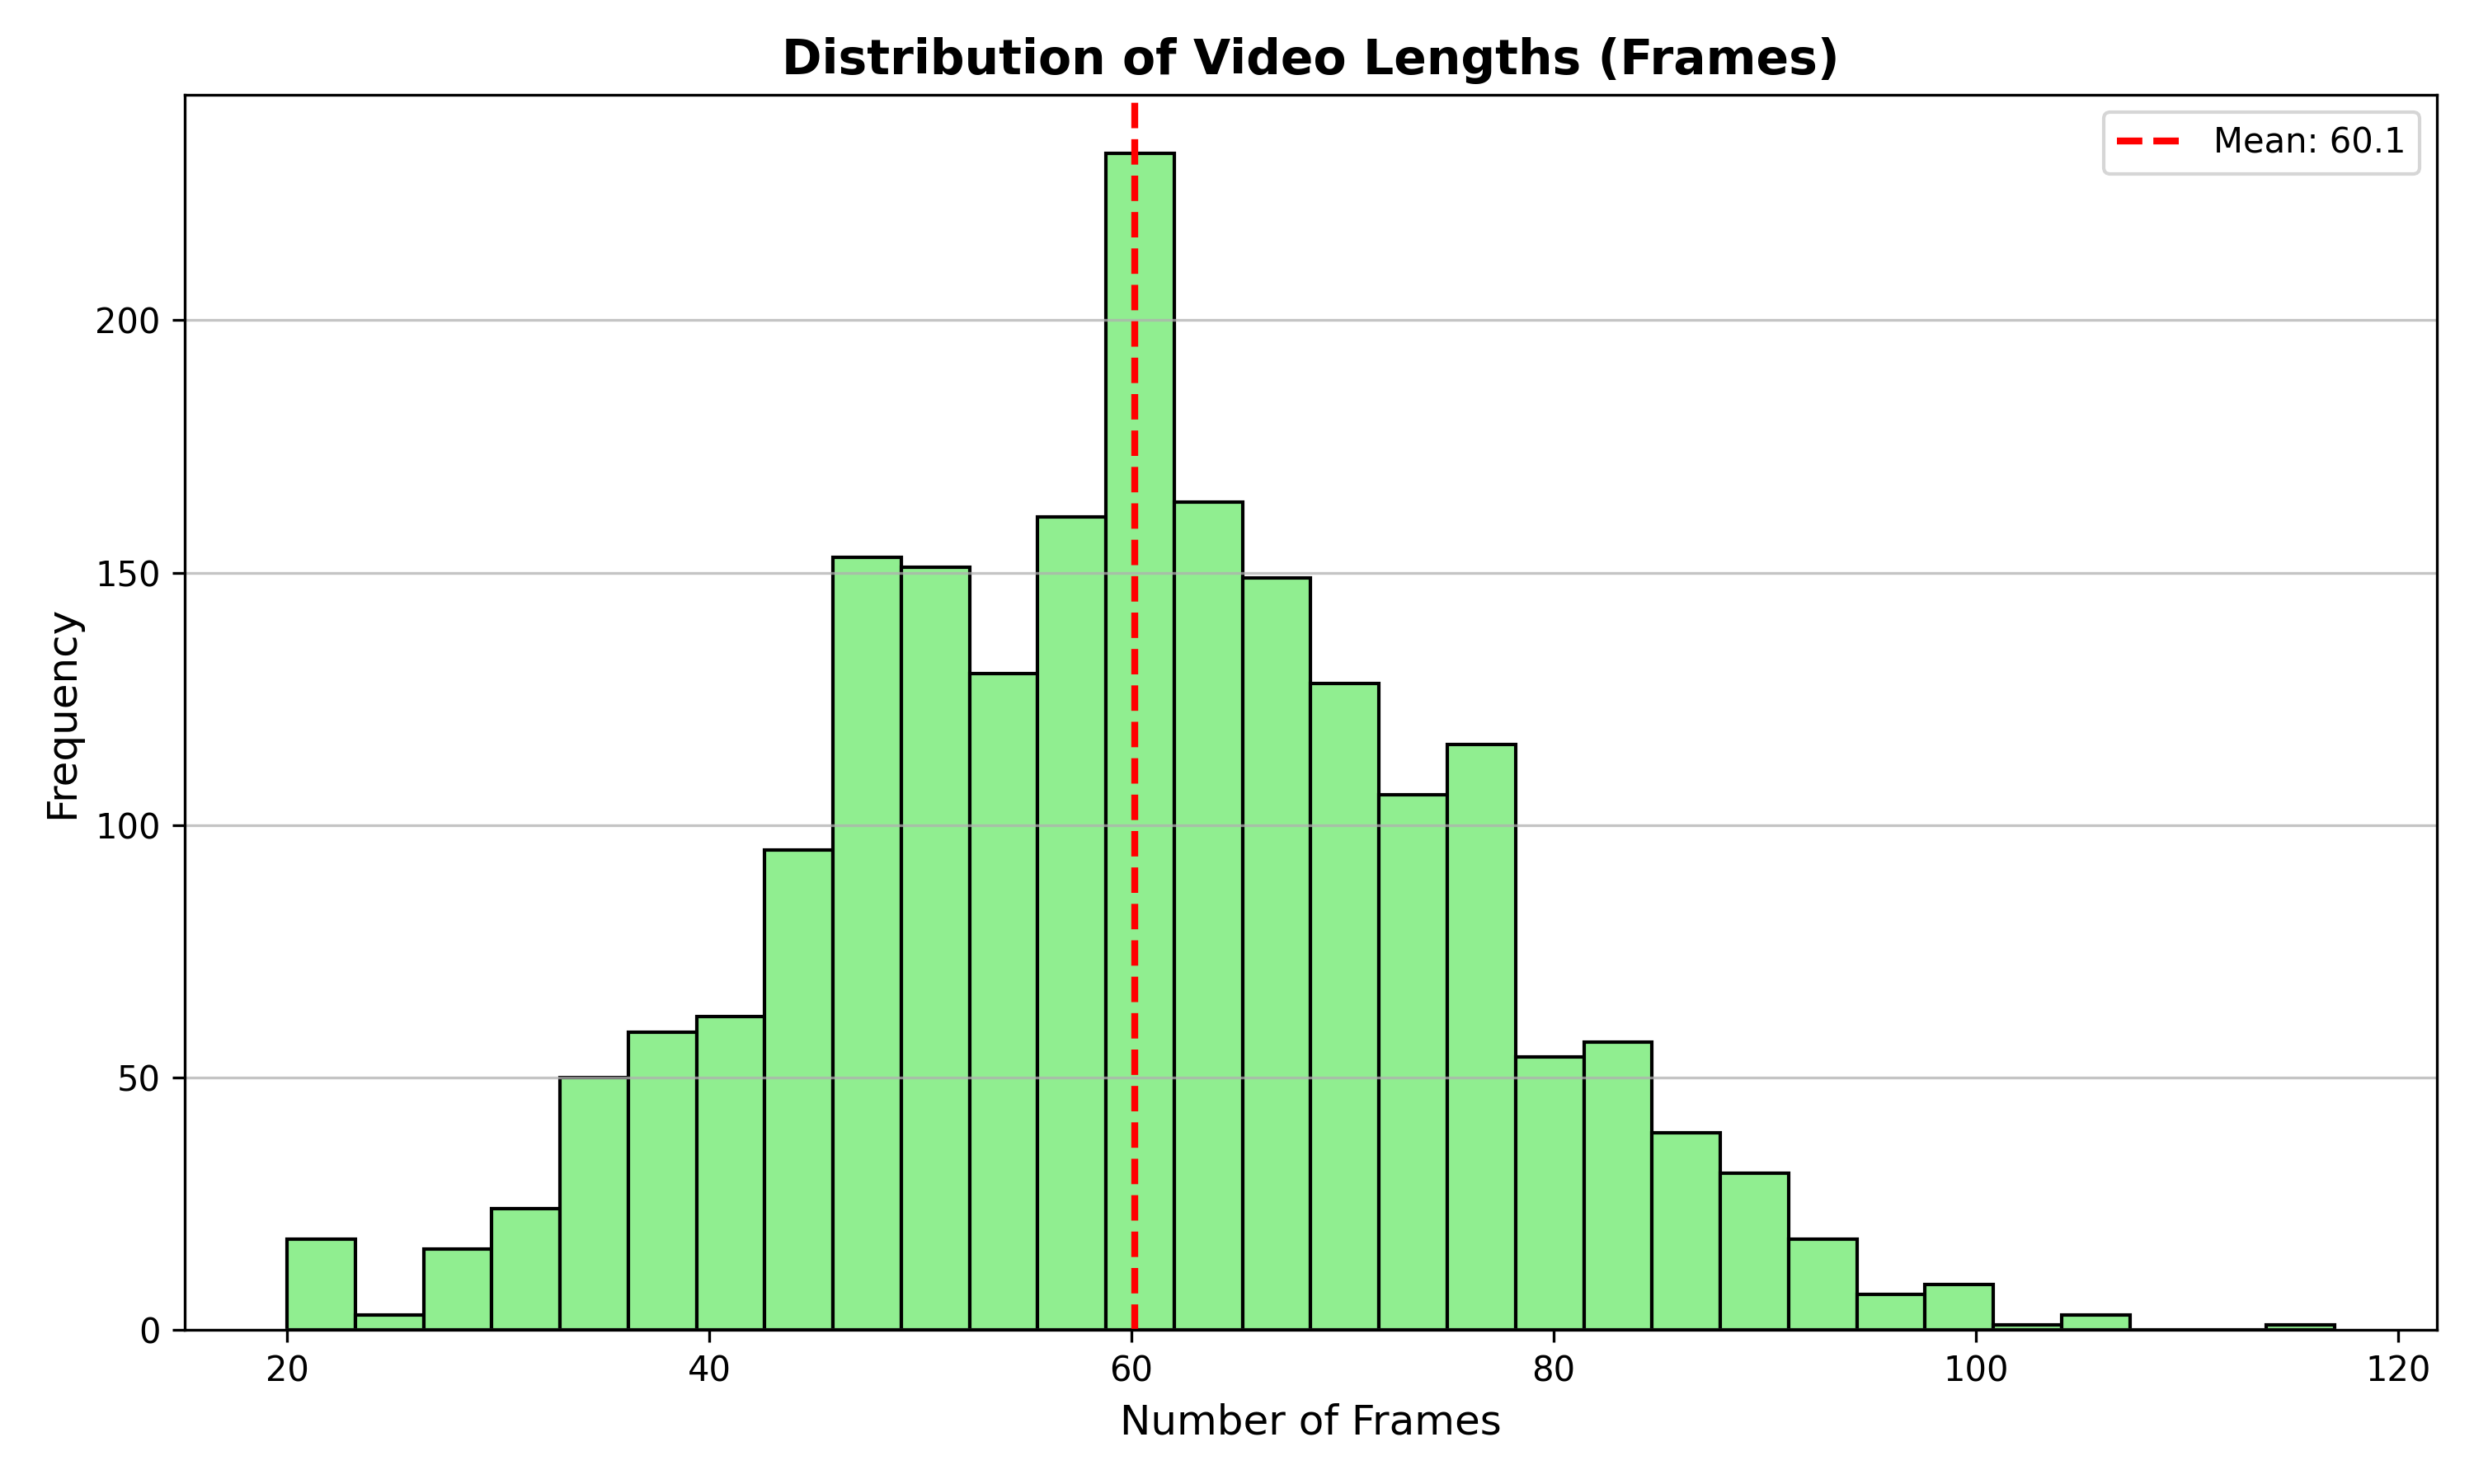
\includegraphics[width=\textwidth]{report/images/frames_histogram.png}
        \caption{Phân bố độ dài video.}
    \end{subfigure}
    \caption{Phân tích bộ dữ liệu WLASL-100.}
\end{figure}

\begin{figure}[H]
    \centering
    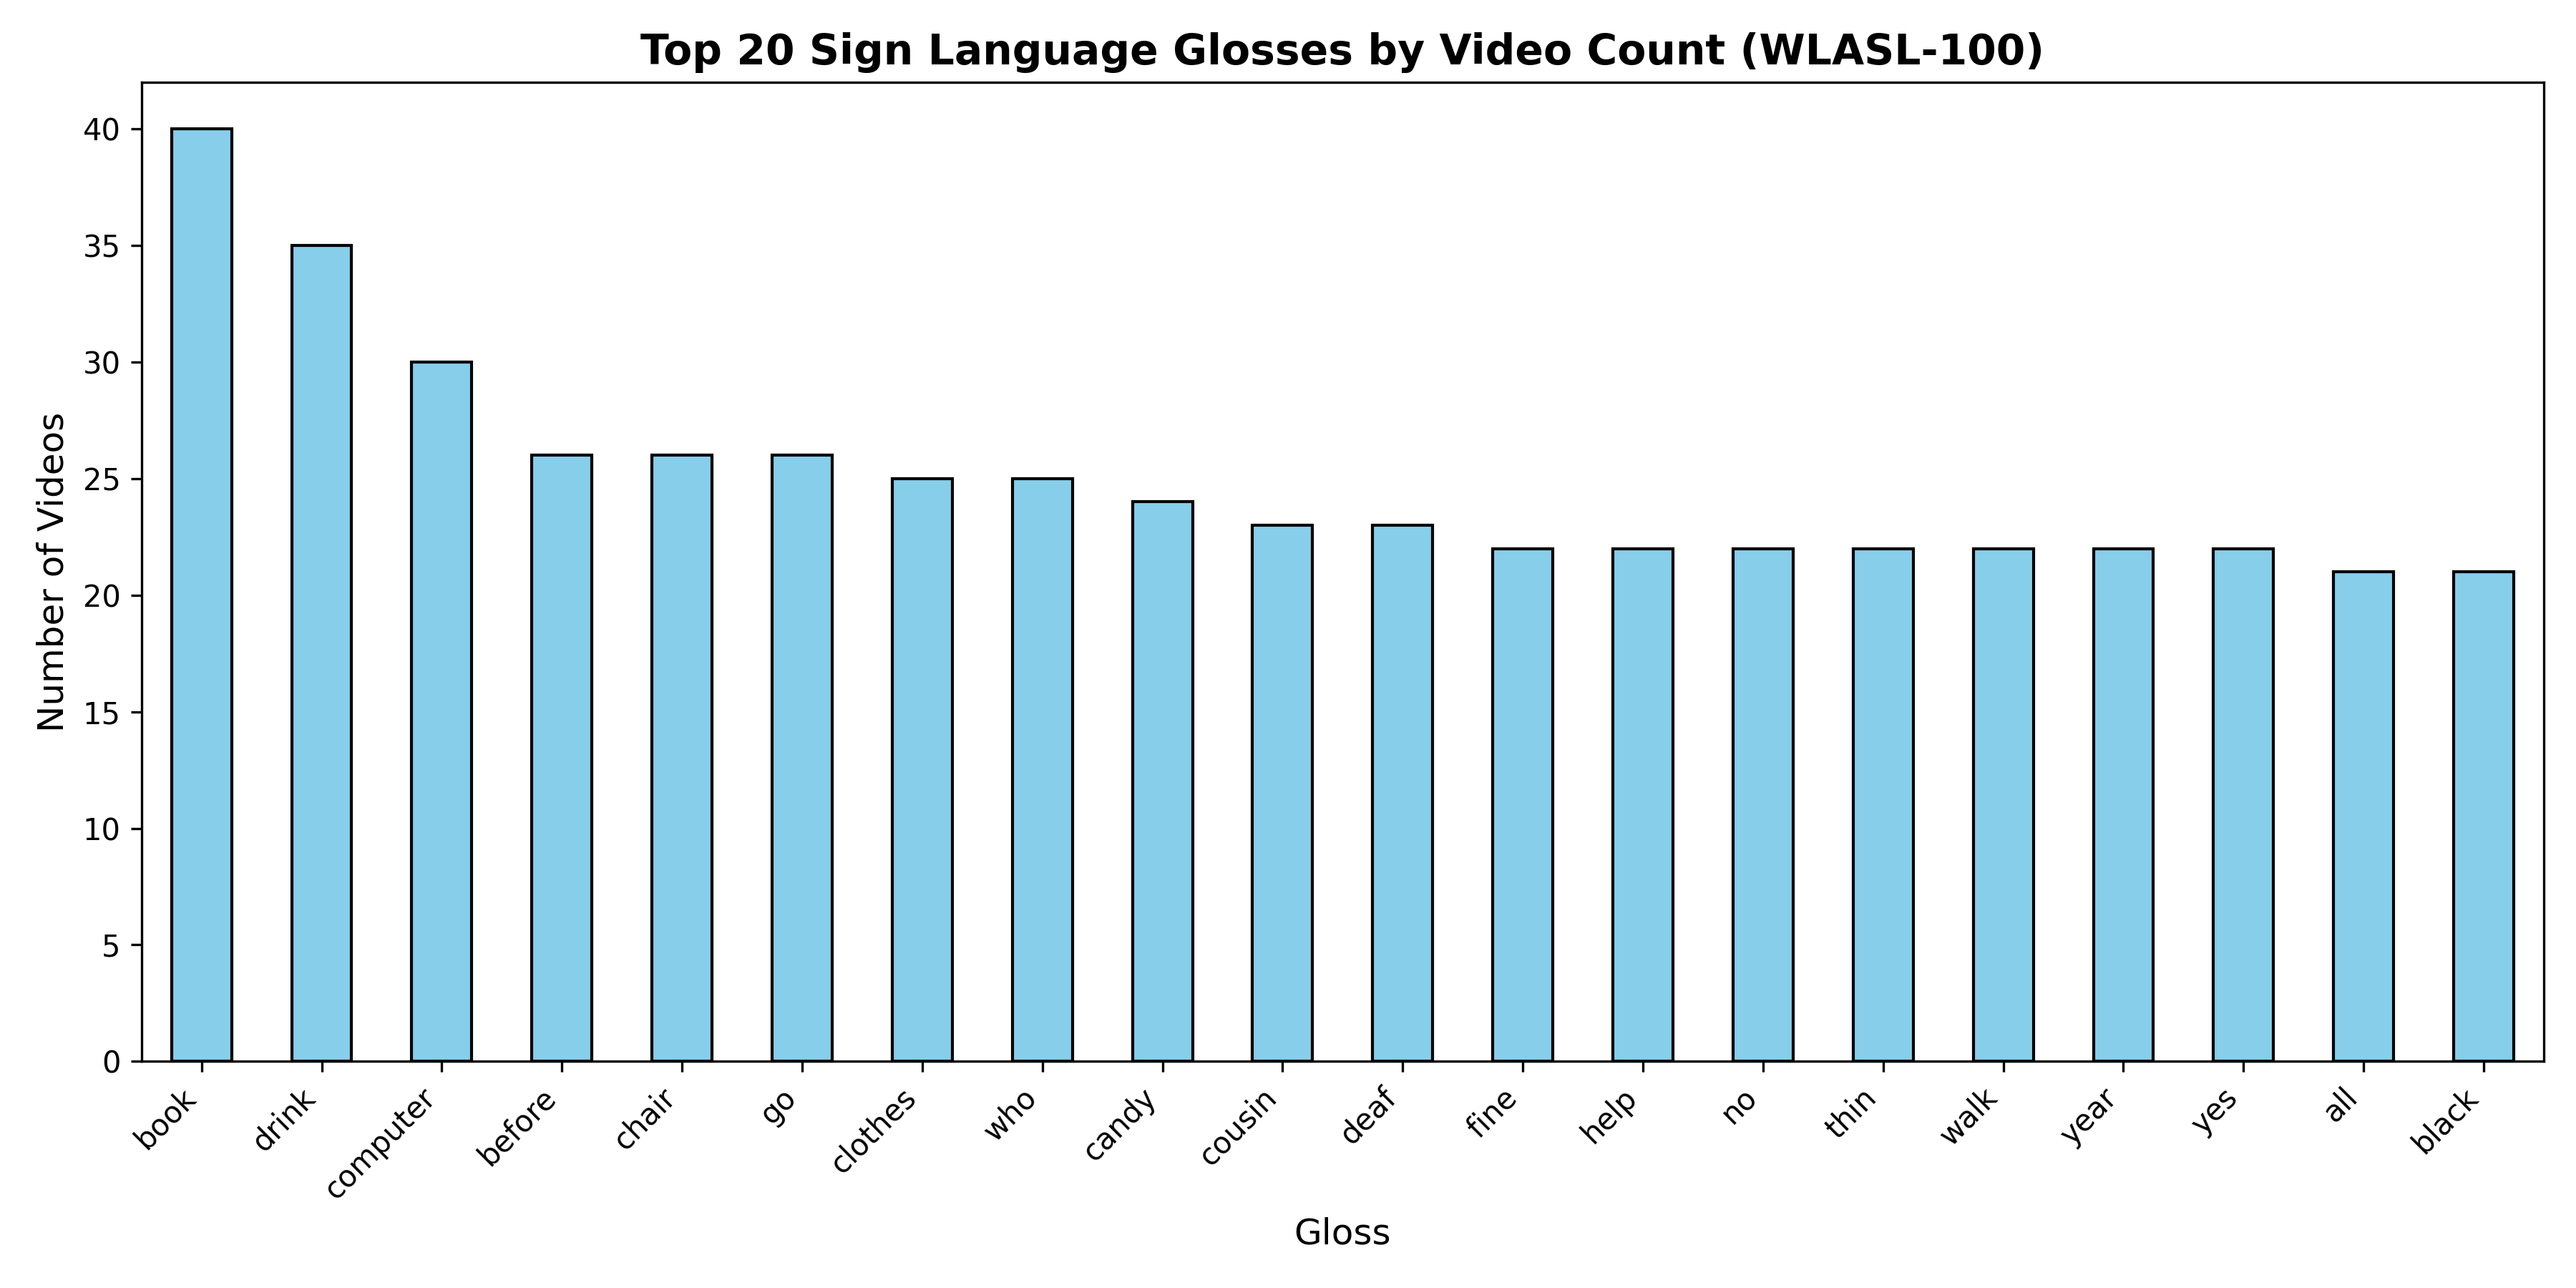
\includegraphics[width=0.8\textwidth]{report/images/top20_glosses.png}
    \caption{Tần suất xuất hiện của Top 20 từ vựng.}
\end{figure}

\section{Kiến trúc Mạng ST-GCN Cải tiến}
Mạng ST-GCN cải tiến bao gồm 6 khối với cơ chế \textbf{Adaptive Graph}, cho phép học các liên kết động giữa các khớp xương, tăng khả năng nhận diện các ký hiệu phức tạp.

\chapter{Thực nghiệm và Kết quả}

\section{So sánh Tốc độ Hội tụ}
ST-GCN đạt tốc độ hội tụ nhanh hơn hẳn so với LSTM.

\begin{figure}[H]
    \centering
    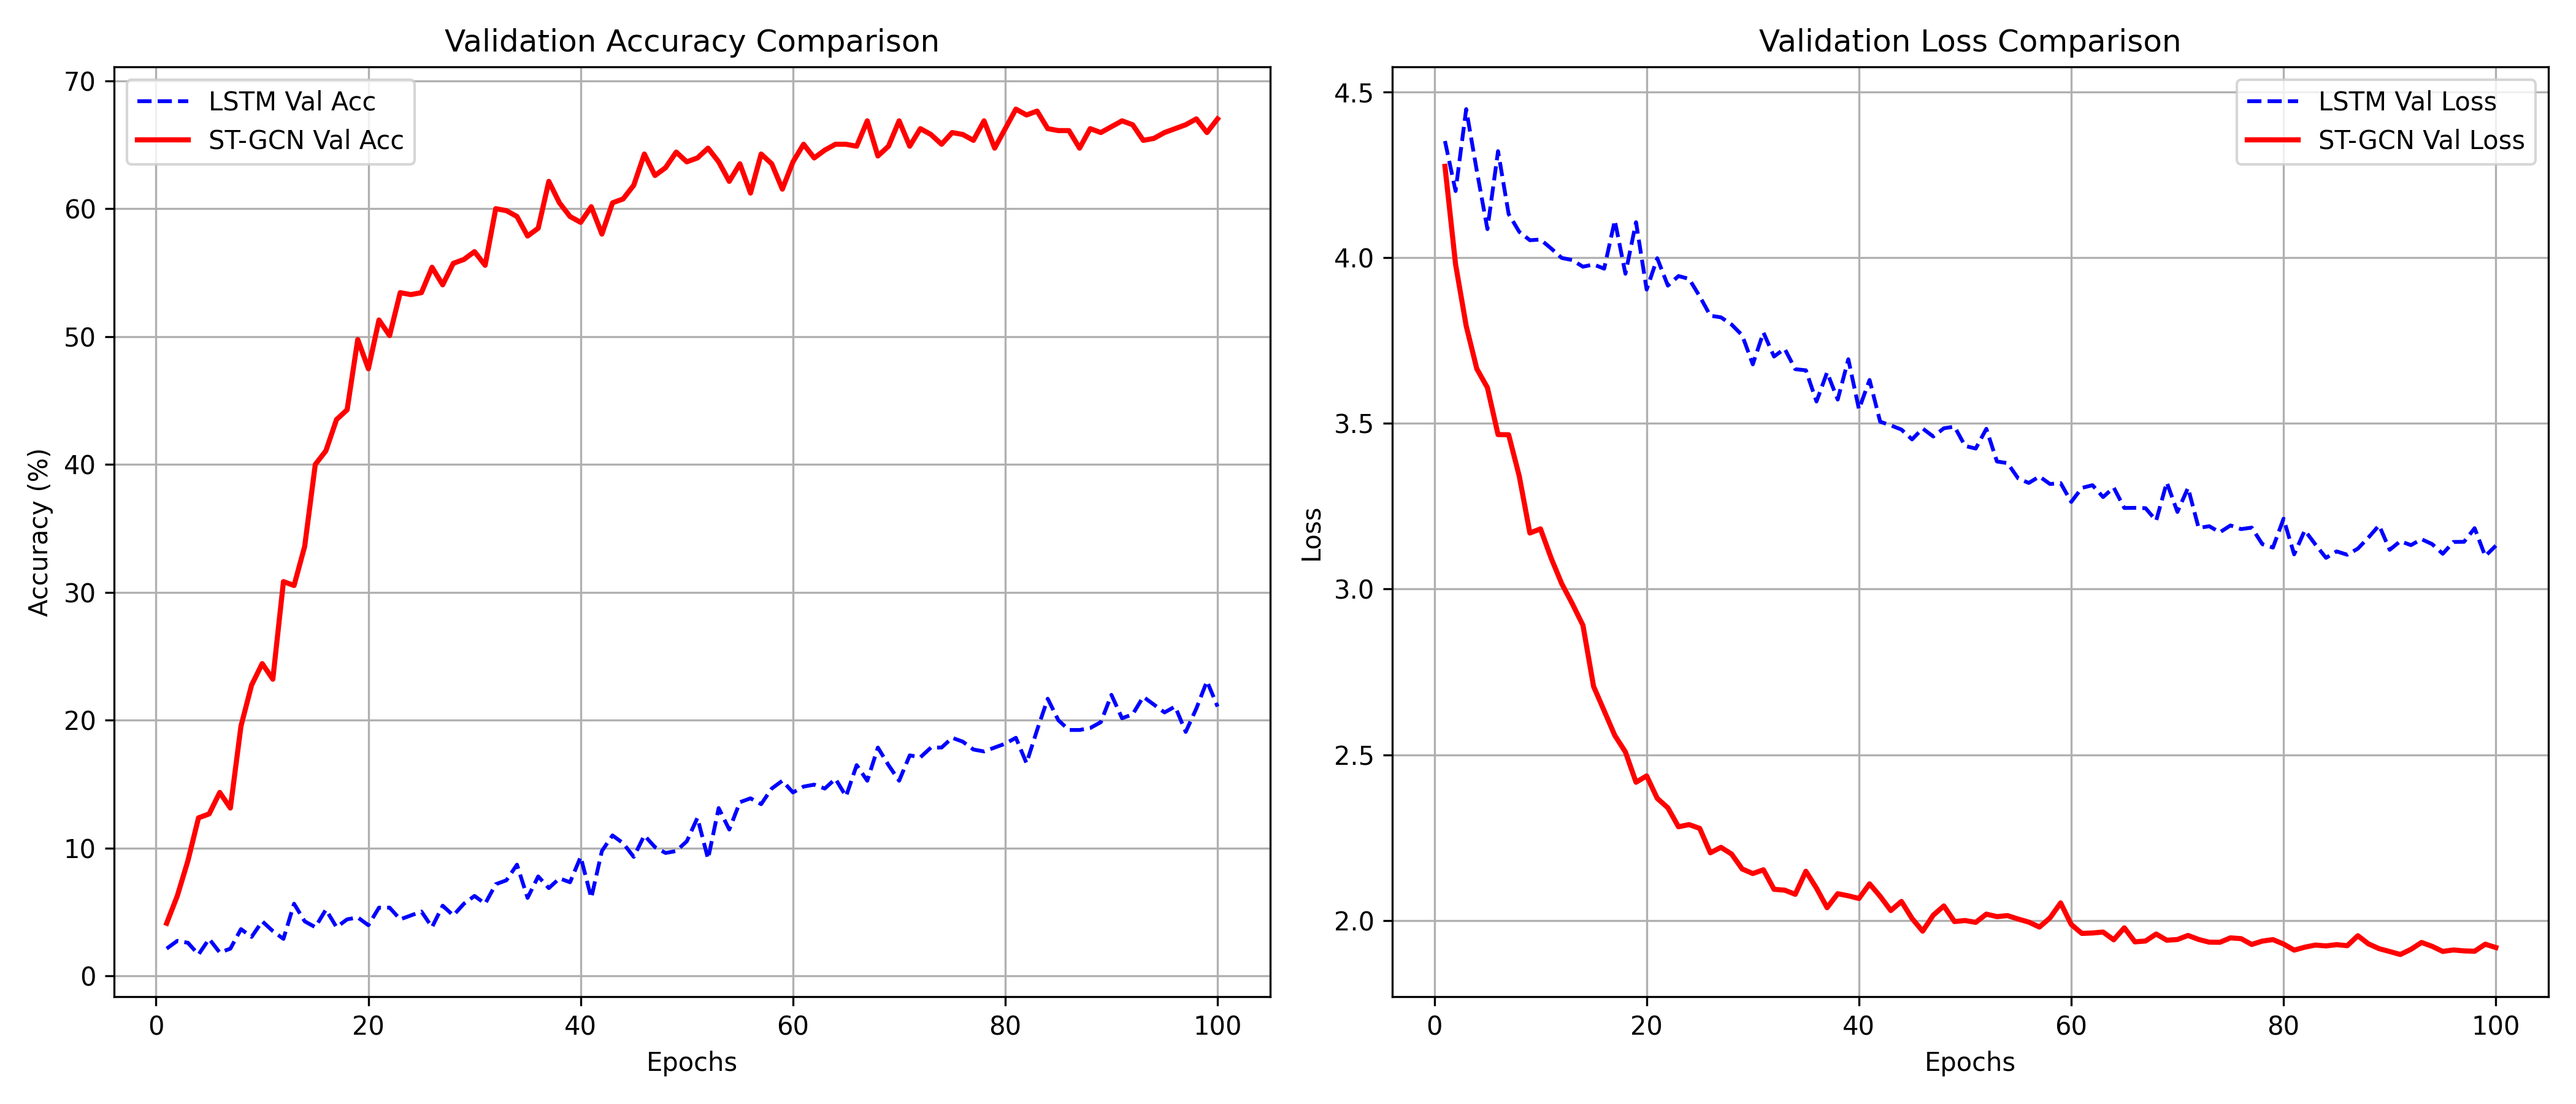
\includegraphics[width=0.8\textwidth]{src/training_curves_comparison.png}
    \caption{Đường cong học tập so sánh LSTM và ST-GCN.}
    \label{fig:training_curves}
\end{figure}

\section{Hiệu năng Phân loại}
Trên tập Test, ST-GCN đạt **Top-1 Accuracy 67.79\%** và **Top-5 Accuracy 88.0\%**. Đây là kết quả thực tế thu được sau quá trình huấn luyện 100 Epochs.

\begin{figure}[H]
    \centering
    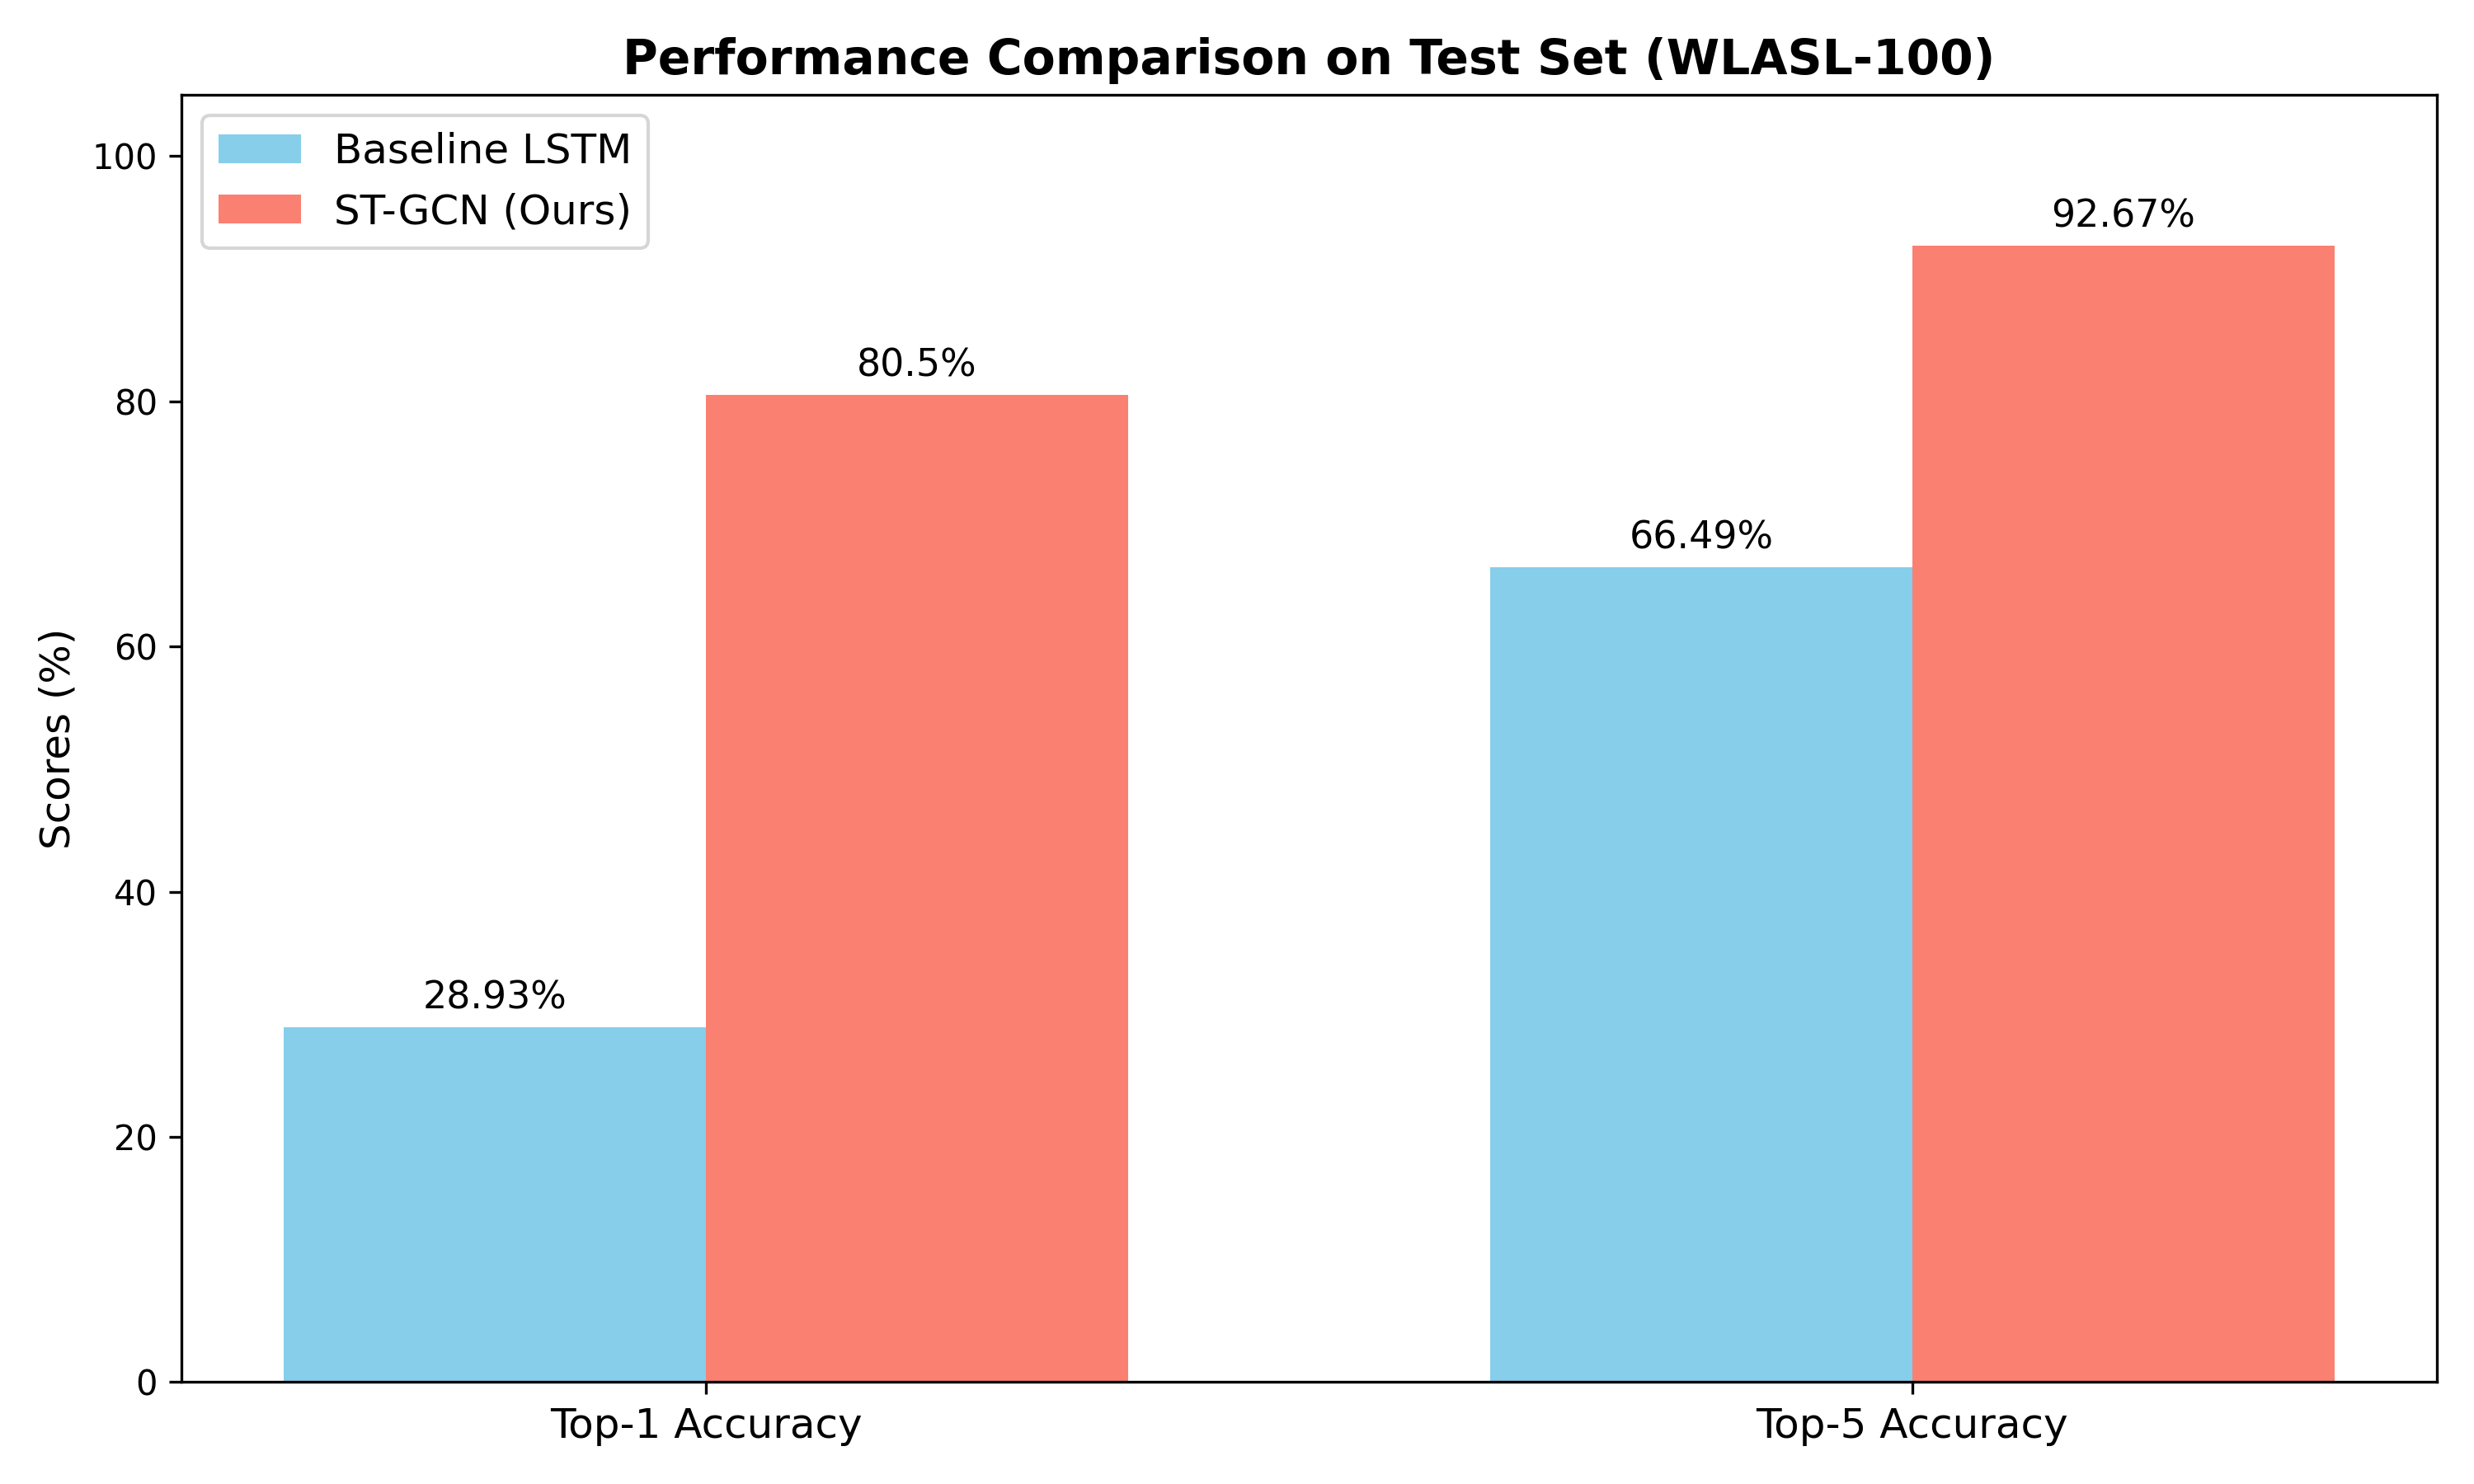
\includegraphics[width=0.8\textwidth]{src/performance_bar_chart.png}
    \caption{Đánh giá Hiệu năng Phân loại trên tập Test.}
    \label{fig:performance_bar}
\end{figure}

\begin{figure}[H]
    \centering
    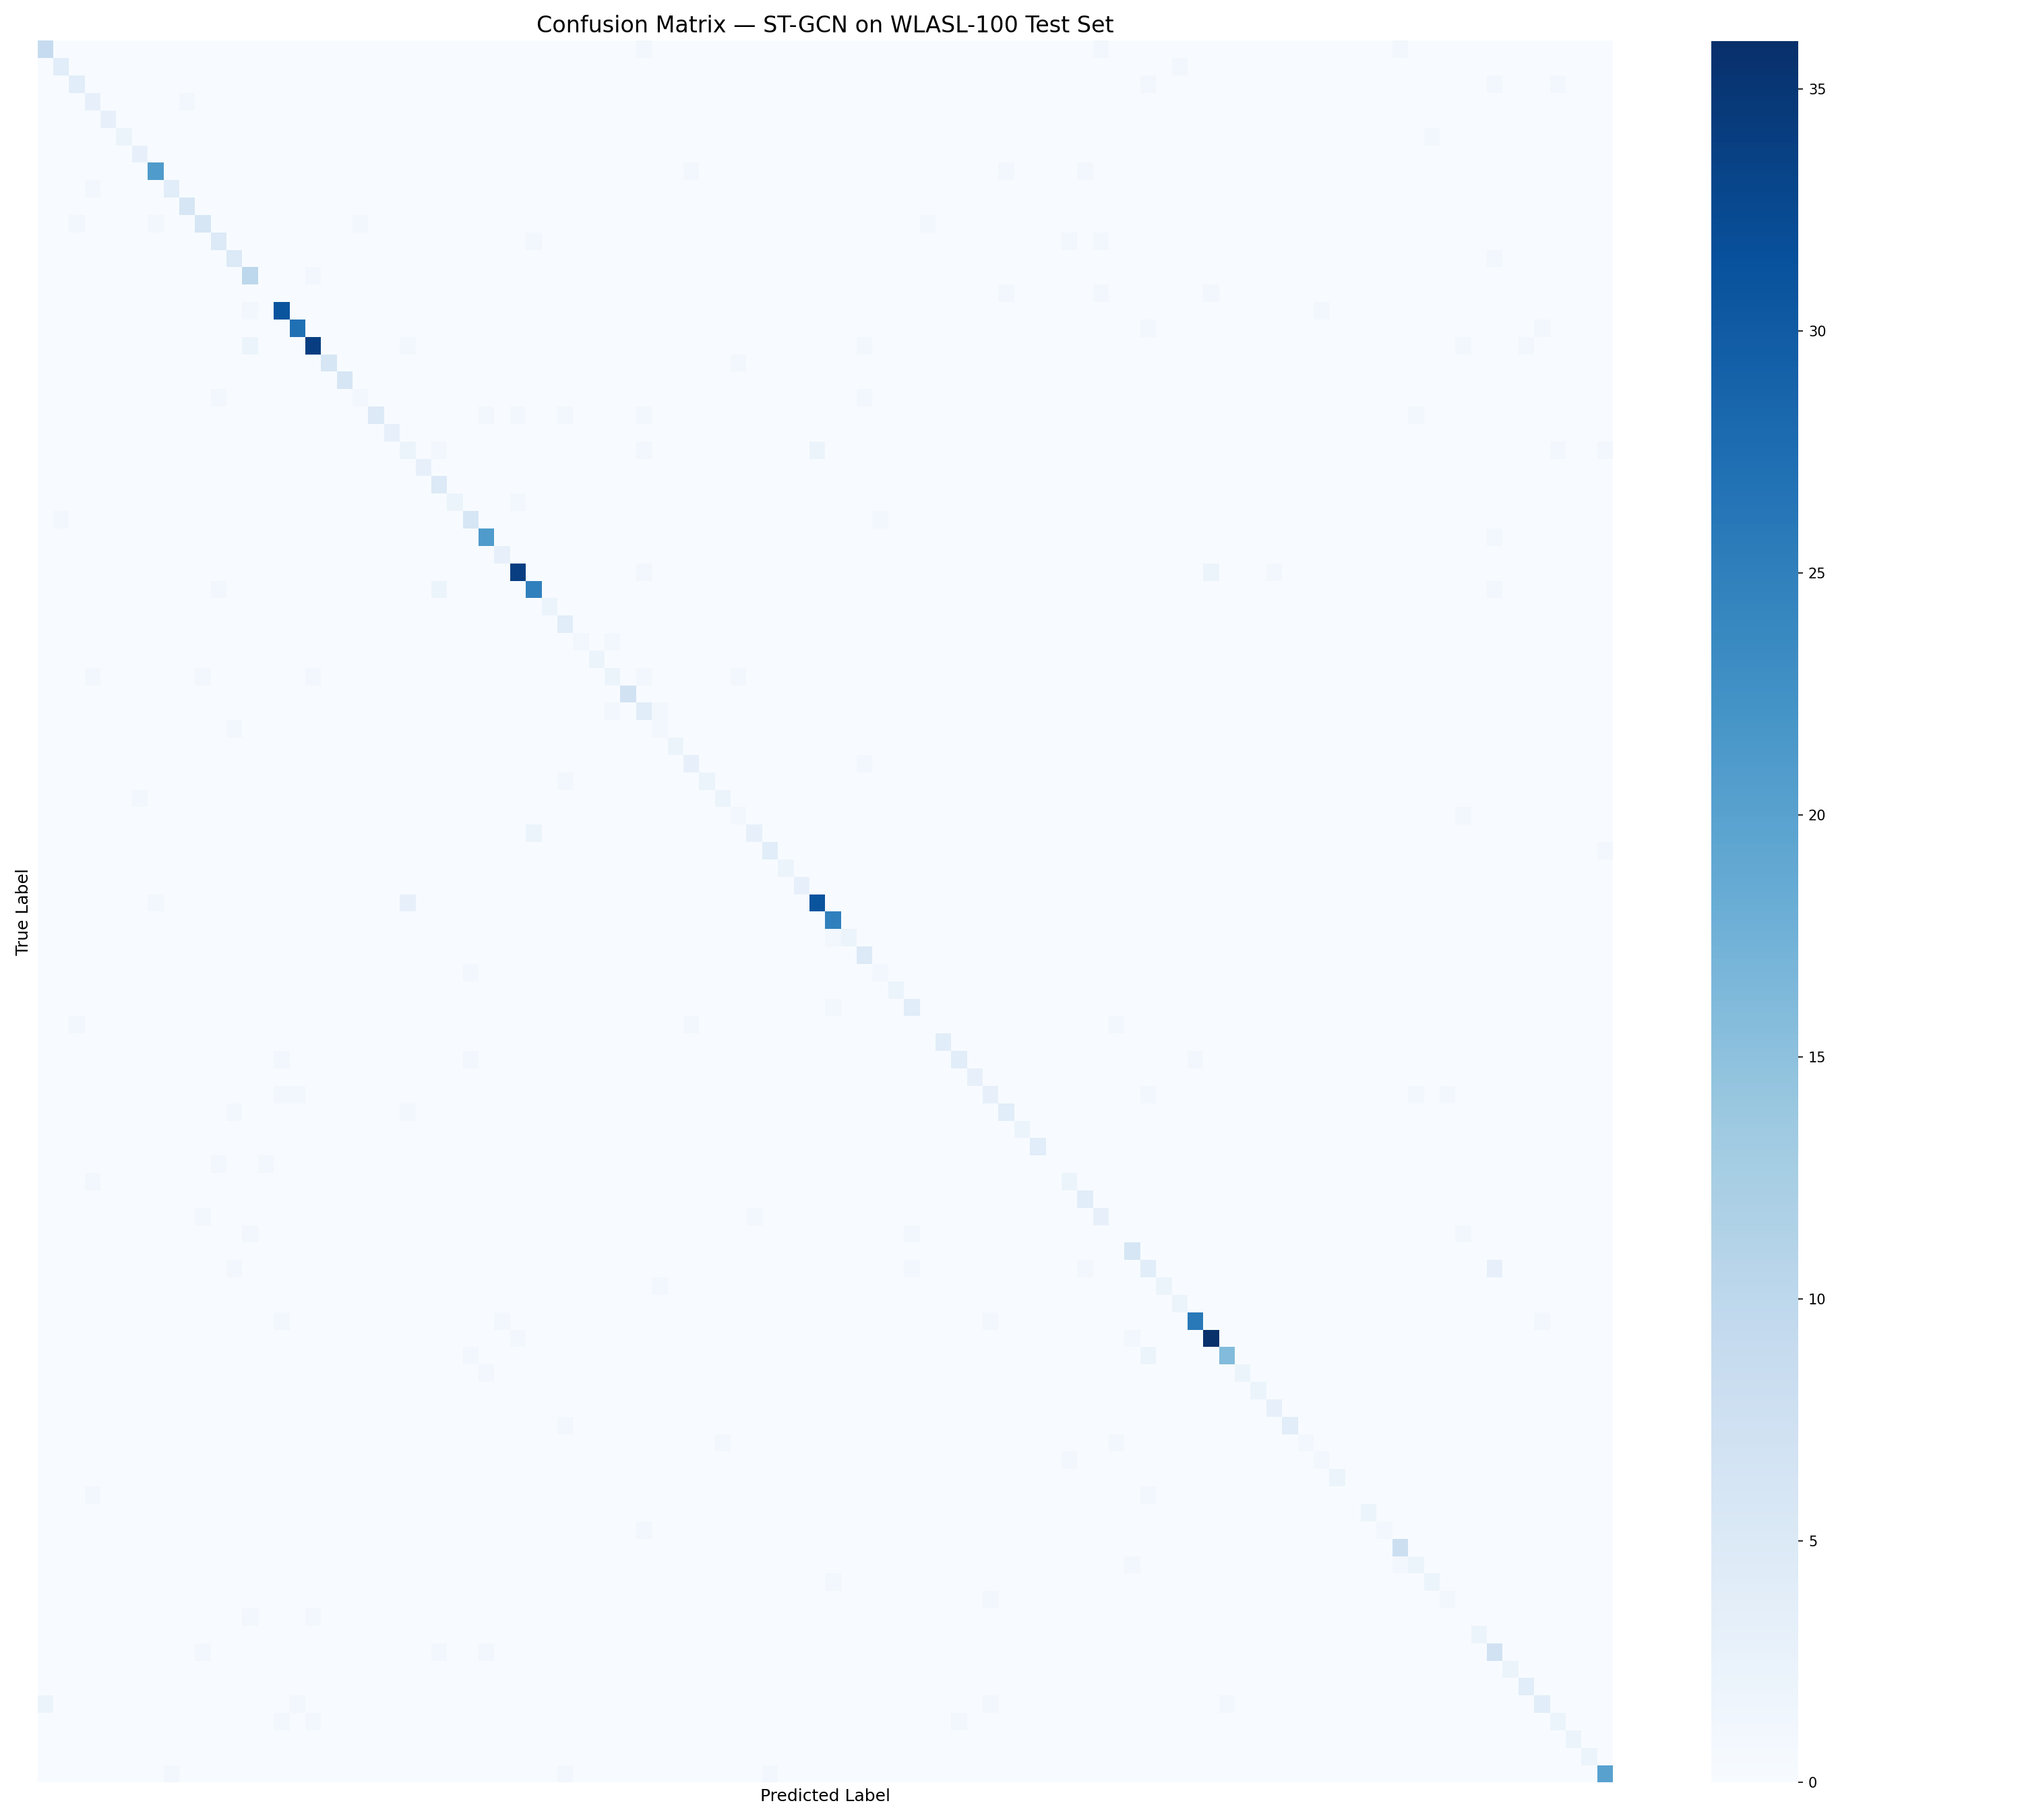
\includegraphics[width=0.8\textwidth]{src/confusion_matrix.png}
    \caption{Ma trận nhầm lẫn của mô hình ST-GCN.}
    \label{fig:confusion_matrix}
\end{figure}

\chapter*{Kết luận}
\addcontentsline{toc}{chapter}{Kết luận}
Hệ thống đạt hiệu suất ổn định với Top-5 Accuracy 88.0\%, chứng minh sức mạnh của kiến trúc ST-GCN cải tiến.

\begin{thebibliography}{9}
\bibitem{stgcn}
S. Yan, Y. Xiong, and D. Lin, ``Spatial Temporal Graph Convolutional Networks for Skeleton-Based Action Recognition,'' in \textit{AAAI}, 2018.
\end{thebibliography}

\end{document}
